\documentclass[11pt]{article}

% ---------------------------------------------------------------------------
% Deliverable 1 - Problem Definition & Data Foundations
% Track B (Research & Development), Course AI-2002 Artificial Intelligence
% Compile on Overleaf: upload main.tex together with the `figures/` folder.
% ---------------------------------------------------------------------------

\usepackage[margin=1in]{geometry}
\usepackage{graphicx}
\usepackage{booktabs}
\usepackage{amsmath}
\usepackage{amssymb}
\usepackage{float}
\usepackage{caption}
\usepackage{subcaption}
\usepackage{enumitem}
\usepackage{xcolor}
\usepackage[hidelinks]{hyperref}

\graphicspath{{figures/}}
\captionsetup{font=small, labelfont=bf}
\setlist{nosep}

\title{\textbf{Neural-Guided Heuristics versus Classical Pathfinding\\ in Dynamic Grid-Mazes}\\[4pt]
\large Deliverable 1 --- Problem Definition \& Data Foundations}
\author{
  Muhammad Abdullah Saeed \and
  Muhammad Hamid Abad \and
  Abdullah Zia
}
\date{AI-2002 Artificial Intelligence --- Track B (Research \& Development)\\ \today}

\begin{document}
\maketitle

\begin{abstract}
\noindent
This report establishes the problem definition and the data foundations for a study
comparing classical A$^\ast$ search (using the Manhattan-distance heuristic) with a
neural-network-guided A$^\ast$ in procedurally generated grid mazes. We motivate why a
learned heuristic is preferable to hand-designed rules, describe a complete and
reproducible data pipeline---generation, ground-truth labelling with Dijkstra's
algorithm, cleaning, and feature engineering---and present an exploratory data
analysis of the resulting dataset of 2{,}000 generated mazes (1{,}876 after cleaning).
The dataset, code, and figures contained here constitute the data-centric foundation on
which the later training and evaluation phases of the project are built.
\end{abstract}

% ===========================================================================
\section{Introduction}
% ===========================================================================
Pathfinding on grids is a classical problem in artificial intelligence and underlies
applications ranging from video-game navigation to warehouse robotics and route
planning. The de-facto standard is A$^\ast$ search \cite{hart1968}, whose efficiency
depends entirely on the quality of the heuristic $h(n)$ it is given. The classical
choice, the Manhattan distance, is admissible but \emph{uninformed about obstacles}:
in a cluttered maze it underestimates the true cost badly and causes A$^\ast$ to expand
a large number of unnecessary nodes.

This project investigates whether a neural network trained to predict the true
shortest-path cost $h^\ast(n)$ can serve as a superior heuristic, reducing the number of
nodes expanded while preserving near-optimal path quality. Deliverable~1 covers
Phase~1 (problem definition) and Phase~2 (data acquisition and preprocessing) of the
project workflow. The central research hypothesis is:

\begin{quote}
\itshape
A trained neural heuristic $h_\theta(n)$ integrated into A$^\ast$ will expand fewer
nodes than the Manhattan-distance heuristic on complex, obstructed grid mazes, while
maintaining high path optimality.
\end{quote}

% ===========================================================================
\section{Phase 1: Problem Definition}
% ===========================================================================

\subsection{Problem Statement}
Classical A$^\ast$ uses a fixed, hand-crafted heuristic that ignores the specifics of the
environment. On open maps the Manhattan distance is excellent, but as obstacle density
grows---as it does in real maze-like domains such as building interiors, cluttered
warehouse floors, or procedurally generated game levels---the gap between the Manhattan
estimate and the true remaining cost widens dramatically. Two concrete pain points
follow:

\begin{enumerate}
  \item \textbf{Wasted computation.} A weak heuristic forces A$^\ast$ to expand far more
  nodes than necessary, increasing run time and memory. In time-critical or
  resource-constrained settings (real-time games, embedded robotic planners) this is the
  dominant cost.
  \item \textbf{No adaptation.} A rule-based heuristic is fixed a priori. It cannot learn
  that this particular class of maze has long dead-end corridors, or that
  \emph{Perlin}-style blob obstacles systematically change the geometry of the optimal
  path. Every environment is treated identically.
\end{enumerate}

The pain point addressed by this project is therefore: \emph{given a class of grid
environments, how can we obtain a heuristic that is both substantially more informed
than Manhattan distance and cheap enough to be evaluated many times during a single
search?}

\subsection{Target Audience and Research Gap}
The primary beneficiaries are:

\begin{itemize}
  \item \textbf{Game-AI and simulation developers} who need fast pathfinding for many
  agents on procedurally generated maps.
  \item \textbf{Robotics and autonomous-systems engineers} planning through cluttered,
  structured environments where hand-tuned heuristics generalise poorly.
  \item \textbf{The AI research community} studying \emph{learned heuristics} and
  \emph{neural-guided search}---a line of work exemplified by Neural A$^\ast$
  \cite{yonetani2021} and learned heuristic functions.
\end{itemize}

The research gap is precise: most learned-heuristic studies report node-expansion gains
but do not systematically characterise how the choice of \emph{environment generator}
and \emph{obstacle density} affects the admissibility--efficiency trade-off. This project
fills that gap by pairing two contrasting procedural generators (a corridor-like
recursive backtracker and a smooth Perlin-noise generator) across a controlled grid of
sizes and densities, and evaluating a learned heuristic against Manhattan A$^\ast$ and
the exact (oracle) heuristic on that grid.

\subsection{AI Justification}
Why is machine learning necessary here rather than a better rule-based heuristic? The
target function $h^\ast(n)$, the exact cost from a cell to the goal, is the solution of a
shortest-path problem and, in general, has no closed form. Crucially, it is
\emph{environment-dependent}: the same local wall pattern implies very different
remaining costs depending on the global topology of the maze. Hand-designed rules can
only encode local features (Manhattan distance, obstacle penalties, tie-breaking), and
any such rule must remain safely optimistic to preserve admissibility, which caps how
much information it can encode.

A supervised learning approach overcomes this because:

\begin{enumerate}
  \item \textbf{The target is readily available and exact.} For any generated maze we can
  compute $h^\ast(n)$ for every cell with a single Dijkstra search run outward from the
  goal (Section~\ref{sec:labels}). This provides virtually unlimited, perfectly labelled
  training data at negligible cost.
  \item \textbf{The mapping is learnable but not hand-codable.} The remaining cost is a
  smooth function of local geometry and the goal offset; a feed-forward network can
  approximate it far beyond what any fixed rule captures, while a rule cannot be written
  explicitly.
  \item \textbf{Search efficiency is improved by a sharper, not merely admissible,
  estimate.} A$^\ast$ expands nodes with $f(n)=g(n)+h(n)$ below the optimal cost; a
  heuristic that is closer to $h^\ast$ prunes more of the space. Learning to approximate
  $h^\ast$ directly targets this quantity.
\end{enumerate}

A feed-forward neural regressor is therefore the natural tool: it generalises across
mazes, is fast enough at inference to be called inside A$^\ast$, and can be trained
purely from automatic exact labels. The remainder of the project will quantify the
resulting node-expansion reduction and the associated optimality cost.

% ===========================================================================
\section{Phase 2: Data Acquisition and Preprocessing}
% ===========================================================================
Because the domain is synthetic and fully controllable, we adopt a \emph{generation-based}
collection strategy: rather than scraping data, we procedurally generate a large,
balanced, and reproducible dataset, then derive exact labels for it. All stages are
implemented as scripts in \texttt{data\_scripts/} and are governed by a single fixed seed
(42), so the entire dataset can be regenerated bit-for-bit.

\subsection{Data Collection: Maze Generation}
We generate 2{,}000 mazes as the full cross-product of two generators, five grid sizes,
four obstacle densities, and 50 mazes per configuration
($2 \times 5 \times 4 \times 50 = 2{,}000$). The grid convention is
$0=\text{free}$, $1=\text{wall}$.

\begin{itemize}
  \item \textbf{Recursive Backtracker} (\texttt{backtracker}): an iterative depth-first
  search that carves a perfect maze, producing long corridors and dead ends.
  \item \textbf{Perlin Noise} (\texttt{perlin}): fractal gradient noise thresholded so a
  target fraction of cells become walls, producing smooth, connected blobs.
\end{itemize}

Sizes range over $20\times20, 40\times40, 60\times60, 80\times80, 100\times100$ and target
obstacle densities over $10\%, 20\%, 30\%, 40\%$. For each maze a start and a goal are
sampled uniformly from the free cells and constrained to be at least $\text{size}/2$
apart (Manhattan), guaranteeing non-trivial problems. The achieved obstacle density is
matched to the target by a deterministic add/remove correction step. Generation
parameters and per-configuration statistics are recorded in
\texttt{generation\_log.json}.

\subsection{Ground-Truth Labelling}
\label{sec:labels}
For every maze we need the exact cost $h^\ast(n)$ from \emph{every} cell to the goal.
Exploiting the fact that the maze is undirected with unit move cost, a \emph{single}
Dijkstra search run \emph{from the goal} yields $h^\ast(n)$ for all cells
simultaneously---far cheaper than one search per cell. Cells that are walls or that cannot
reach the goal receive $h^\ast(n)=\infty$. The optimal start-to-goal cost is then simply
\texttt{opt\_cost} $= h^\ast(\text{start})$. This stage is implemented in
\texttt{compute\_labels.py}. Of the 2{,}000 mazes, 88 have an unreachable goal
(\texttt{opt\_cost} $=\infty$), and across all mazes 195{,}373 free cells cannot reach
their goal.

\subsection{Data Cleaning}
\label{sec:cleaning}
The cleaning stage (\texttt{clean\_data.py}) enforces data quality along four axes and is
summarised in Table~\ref{tab:cleaning} and Figure~\ref{fig:cleaning}.

\begin{enumerate}
  \item \textbf{Unreachable paths.} Any maze whose \texttt{opt\_cost} is infinite is
  dropped entirely, since it provides no valid learning signal. Within retained mazes,
  invalid cells ($h^\ast=\infty$, i.e.\ walls and unreachable free cells) are marked with
  the sentinel value $-1$ so downstream code can exclude them cleanly.
  \item \textbf{Deduplication.} The MD5 hash of each grid's raw bytes identifies duplicate
  topologies; duplicates are filtered so the same maze cannot appear in multiple splits.
  \item \textbf{Outlier filtering.} For each grid size, extreme optimal path costs are
  flagged using the $\text{IQR}$ rule: a maze is dropped if $\text{opt\_cost} < Q_1 - 1.5\,\text{IQR}$
  or $\text{opt\_cost} > Q_3 + 1.5\,\text{IQR}$. Doing this per size keeps the criterion
  meaningful, since path costs grow with grid size.
  \item \textbf{Logging.} Before/after counts and the per-size IQR bounds are written to
  \texttt{clean\_log.json}.
\end{enumerate}

\begin{table}[H]
\centering
\caption{Data cleaning summary. Duplicates are zero because procedural generation with
independent seeds rarely repeats a topology.}
\label{tab:cleaning}
\begin{tabular}{lrr}
\toprule
Stage & Mazes & Fraction \\
\midrule
Initial (generated)          & 2000 & 100.0\% \\
Dropped: unreachable goal    & 88   & 4.4\%   \\
Dropped: duplicate topology  & 0    & 0.0\%   \\
Dropped: IQR outlier         & 36   & 1.8\%   \\
\midrule
\textbf{Final (cleaned)}     & \textbf{1876} & \textbf{93.8\%} \\
\bottomrule
\end{tabular}
\end{table}

\begin{table}[H]
\centering
\caption{Per-size IQR outlier bounds on optimal path cost (cells).}
\label{tab:iqr}
\begin{tabular}{rrrrrr}
\toprule
Size & $Q_1$ & $Q_3$ & IQR & Lower bound & Upper bound \\
\midrule
20  & 14 & 23 & 9  & 0.5  & 36.5  \\
40  & 27 & 42 & 15 & 4.5  & 64.5  \\
60  & 42 & 63 & 21 & 10.5 & 94.5  \\
80  & 57 & 87 & 30 & 12.0 & 132.0 \\
100 & 71 & 107 & 36 & 17.0 & 161.0 \\
\bottomrule
\end{tabular}
\end{table}

\subsection{Feature Engineering}
\label{sec:features}
For every \emph{reachable} free cell the feature vector $\mathbf{x}(n)\in\mathbb{R}^{29}$
is constructed (\texttt{features.py}) as follows:

\begin{enumerate}
  \item \textbf{Normalised coordinates} $(x/N,\,y/N)\in[0,1]^2$ ($2$ features), where
  $N$ is the grid side length.
  \item \textbf{Goal-relative offset} $(\Delta x/N,\,\Delta y/N)$ with
  $\Delta x = x - x_{\text{goal}}$, giving a vector in $(-1,1)^2$ that tells the network
  where the goal is relative to the current cell ($2$ features).
  \item \textbf{Local wall context.} A $5\times5$ binary window centred on the cell,
  flattened to $25$ features. Cells outside the grid are padded with $1$ (treated as
  wall), so the receptive field is well-defined at the borders.
\end{enumerate}

The regression target is the normalised ground-truth cost
$y(n) = h^\ast(n)/N \in [0,1]$, which keeps the target scale comparable across grid
sizes. Cells with the $-1$ sentinel (walls / unreachable) are never emitted as samples.

\subsection{Train / Validation / Test Split}
To prevent leakage, the split is performed \emph{by maze}, not by cell: all cells of a
given maze belong to exactly one split, so the model is always evaluated on topologies it
has never seen. A fixed seed drives a $70/15/15$ assignment over the 1{,}876 cleaned
mazes. Table~\ref{tab:split} reports the resulting sizes.

\begin{table}[H]
\centering
\caption{Dataset split by maze and the resulting number of cell samples.}
\label{tab:split}
\begin{tabular}{lrrc}
\toprule
Split & Mazes & Cell samples & Feature dim \\
\midrule
Train & 1313 & 4{,}407{,}160 & 29 \\
Validation & 281 & 896{,}328 & 29 \\
Test & 282 & 911{,}949 & 29 \\
\midrule
\textbf{Total} & \textbf{1876} & \textbf{6{,}215{,}437} & 29 \\
\bottomrule
\end{tabular}
\end{table}

% ===========================================================================
\section{Exploratory Data Analysis}
% ===========================================================================
All figures below are produced by \texttt{eda.py} from the generated, labelled, cleaned,
and feature-engineered data.

\subsection{Obstacle-Density Fidelity}
Figure~\ref{fig:density} compares the target obstacle density of each configuration with
the density actually achieved after the correction step. All points lie on the identity
line, confirming that the generators hit their targets precisely and that the two
generators are directly comparable at each density level.

\begin{figure}[H]
\centering
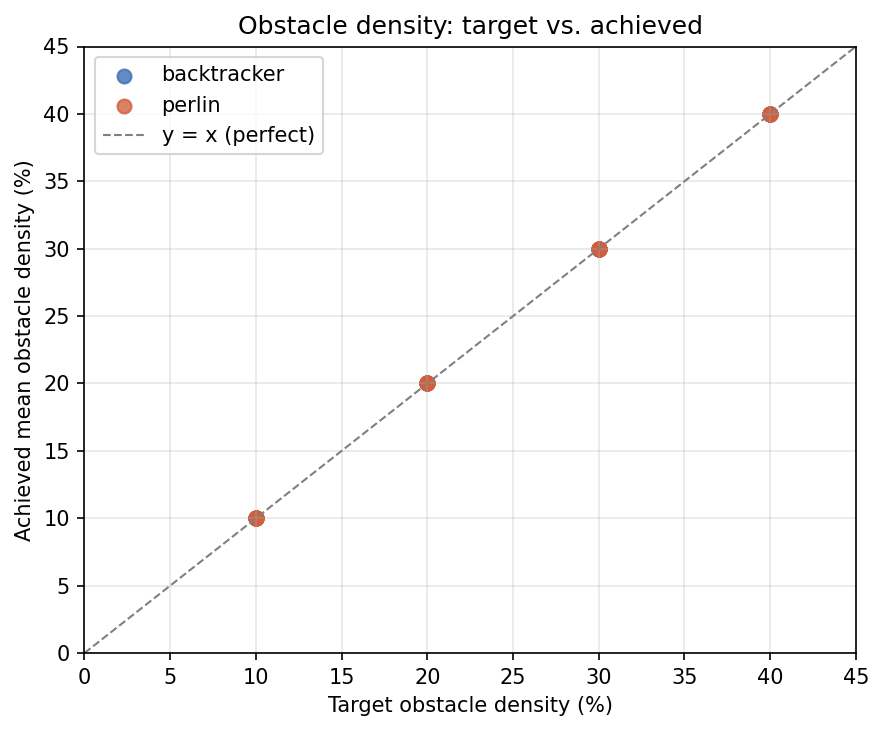
\includegraphics[width=0.62\textwidth]{01_density_target_vs_achieved.png}
\caption{Achieved versus target obstacle density for every configuration.}
\label{fig:density}
\end{figure}

\subsection{Dataset Composition}
Figure~\ref{fig:counts} shows the number of retained mazes per grid size and generator
after cleaning. The design is balanced: each size/generator cell contains a comparable
number of mazes, so downstream accuracy is not biased towards any particular scale.

\begin{figure}[H]
\centering
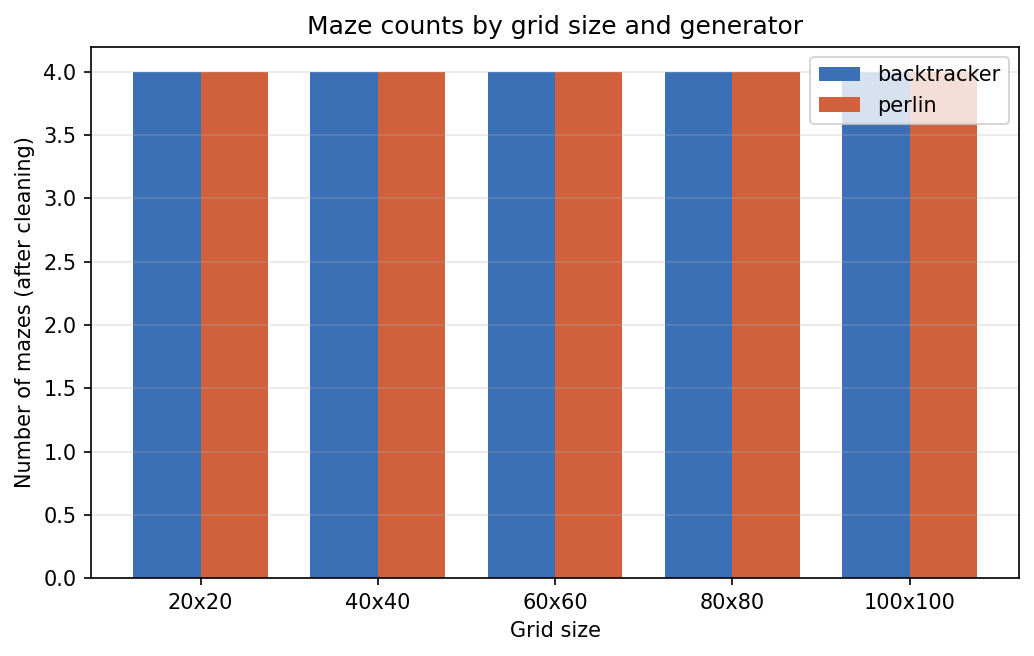
\includegraphics[width=0.7\textwidth]{02_maze_counts.png}
\caption{Number of mazes per grid size and generator after cleaning.}
\label{fig:counts}
\end{figure}

\subsection{Distribution of Optimal Path Costs}
Figure~\ref{fig:optcost} shows the distribution of \texttt{opt\_cost} per grid size. As
expected, both the median and the spread grow with grid size. The per-size spread is
precisely why IQR outlier detection is applied \emph{within} each size rather than
globally: a globally applied threshold would discard many legitimate large-maze instances
while admitting small-maze outliers.

\begin{figure}[H]
\centering
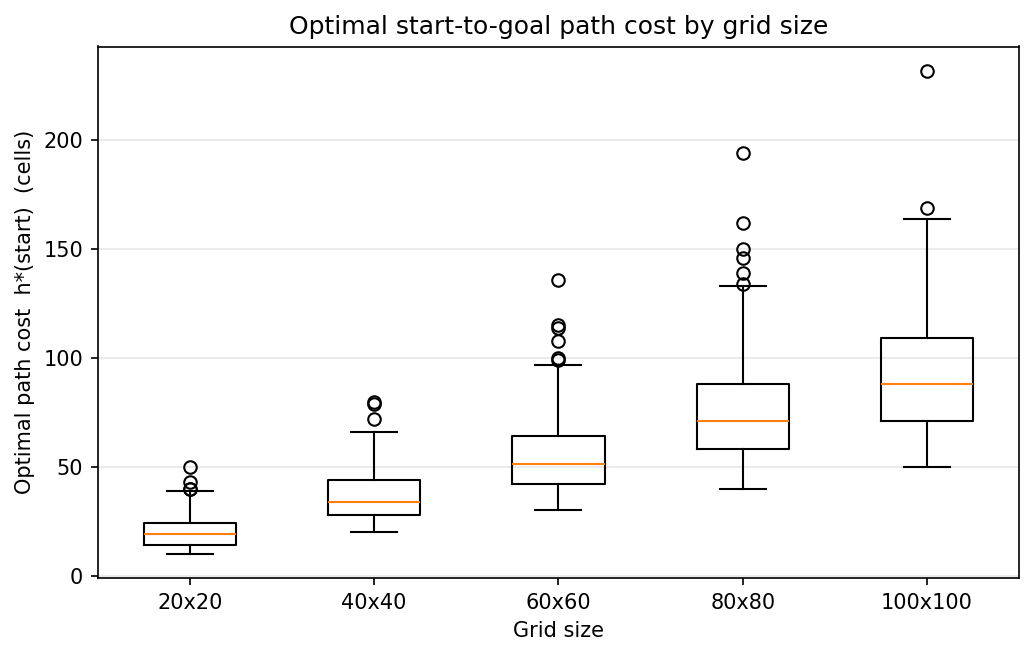
\includegraphics[width=0.7\textwidth]{03_opt_cost_by_size.png}
\caption{Optimal start-to-goal path cost by grid size.}
\label{fig:optcost}
\end{figure}

\subsection{Ground-Truth Heuristic Distribution}
Figure~\ref{fig:hstar} shows the distribution of the \emph{normalised} target
$h^\ast(n)/N$ per grid size. Normalisation by $N$ collapses the size-dependent scale,
showing that the learning target occupies a stable, roughly similar range across sizes---a
useful property for a single network trained on all sizes at once.

\begin{figure}[H]
\centering
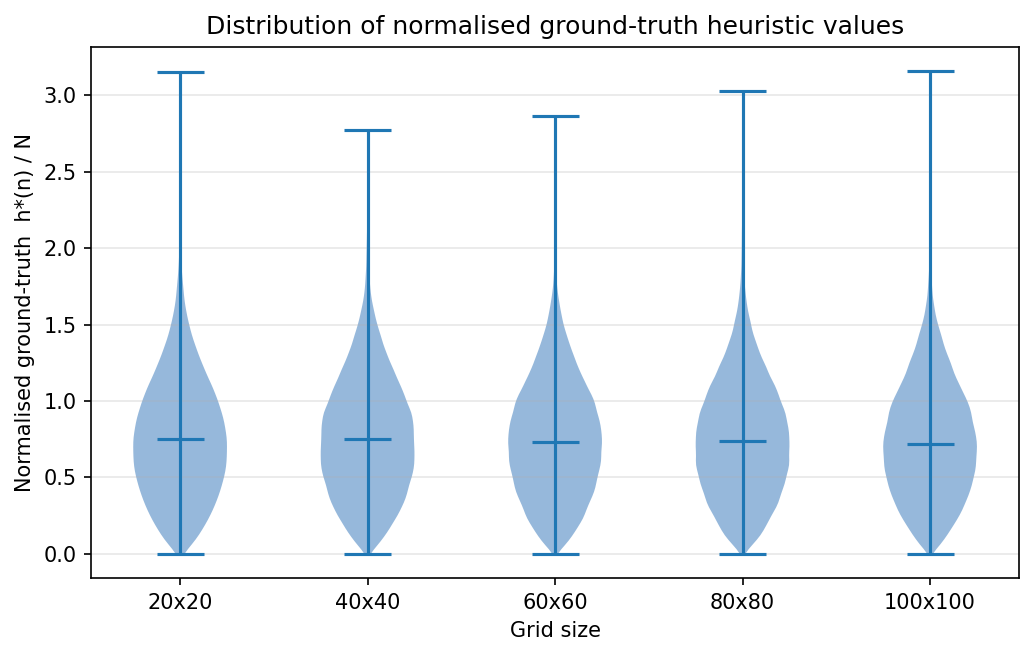
\includegraphics[width=0.7\textwidth]{04_hstar_distribution.png}
\caption{Distribution of the normalised ground-truth heuristic $h^\ast(n)/N$.}
\label{fig:hstar}
\end{figure}

\subsection{Reachability}
Figure~\ref{fig:reach} plots the fraction of free cells that can reach the goal against
obstacle density. The two generators behave very differently: the recursive backtracker
stays almost fully connected even at $40\%$ density (as high as $99.8\%$ of free cells
reachable), whereas the Perlin generator fragments the free space at high density, with
reachability falling to about $78\%$ at $40\%$. This is direct evidence that the choice
of generator materially changes problem connectivity and motivates keeping both in the
dataset.

\begin{figure}[H]
\centering
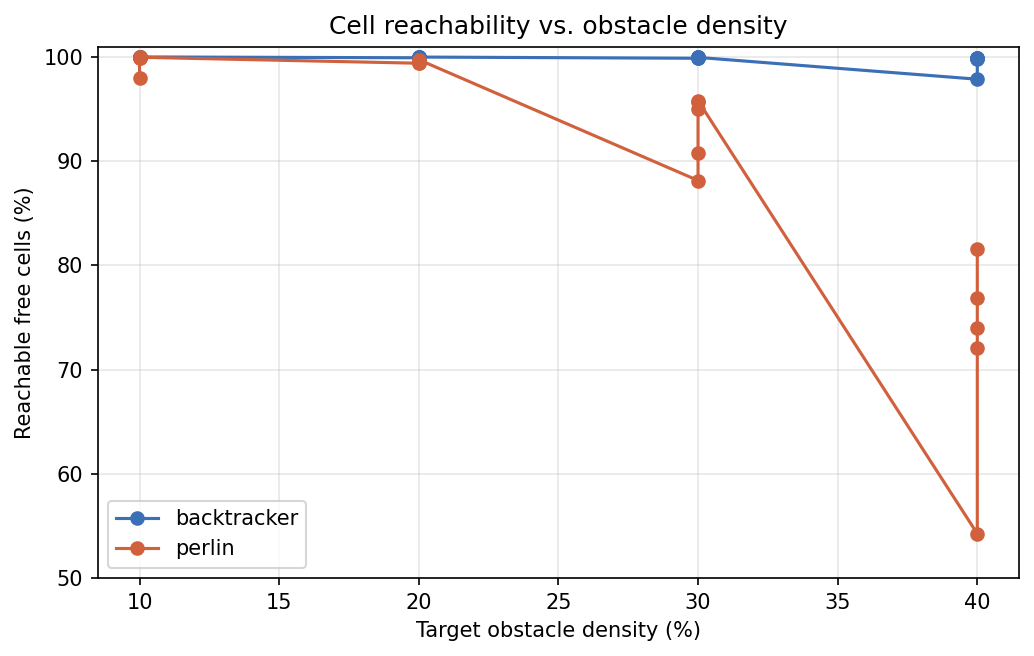
\includegraphics[width=0.7\textwidth]{05_reachable_fraction.png}
\caption{Reachable free cells versus obstacle density, by generator.}
\label{fig:reach}
\end{figure}

\subsection{Sample Mazes and Ground-Truth Fields}
Figure~\ref{fig:samples} visualises representative mazes together with the
ground-truth distance field $h^\ast(n)$ (darker cells are farther from the goal) and the
start/goal positions. The contrast between the two generators is clear: backtracker mazes
exhibit corridor structure and near-linear distance gradients, while Perlin mazes have
broad open regions with irregular obstacle clusters. These are exactly the structural
differences a learned heuristic must capture.

\begin{figure}[H]
\centering
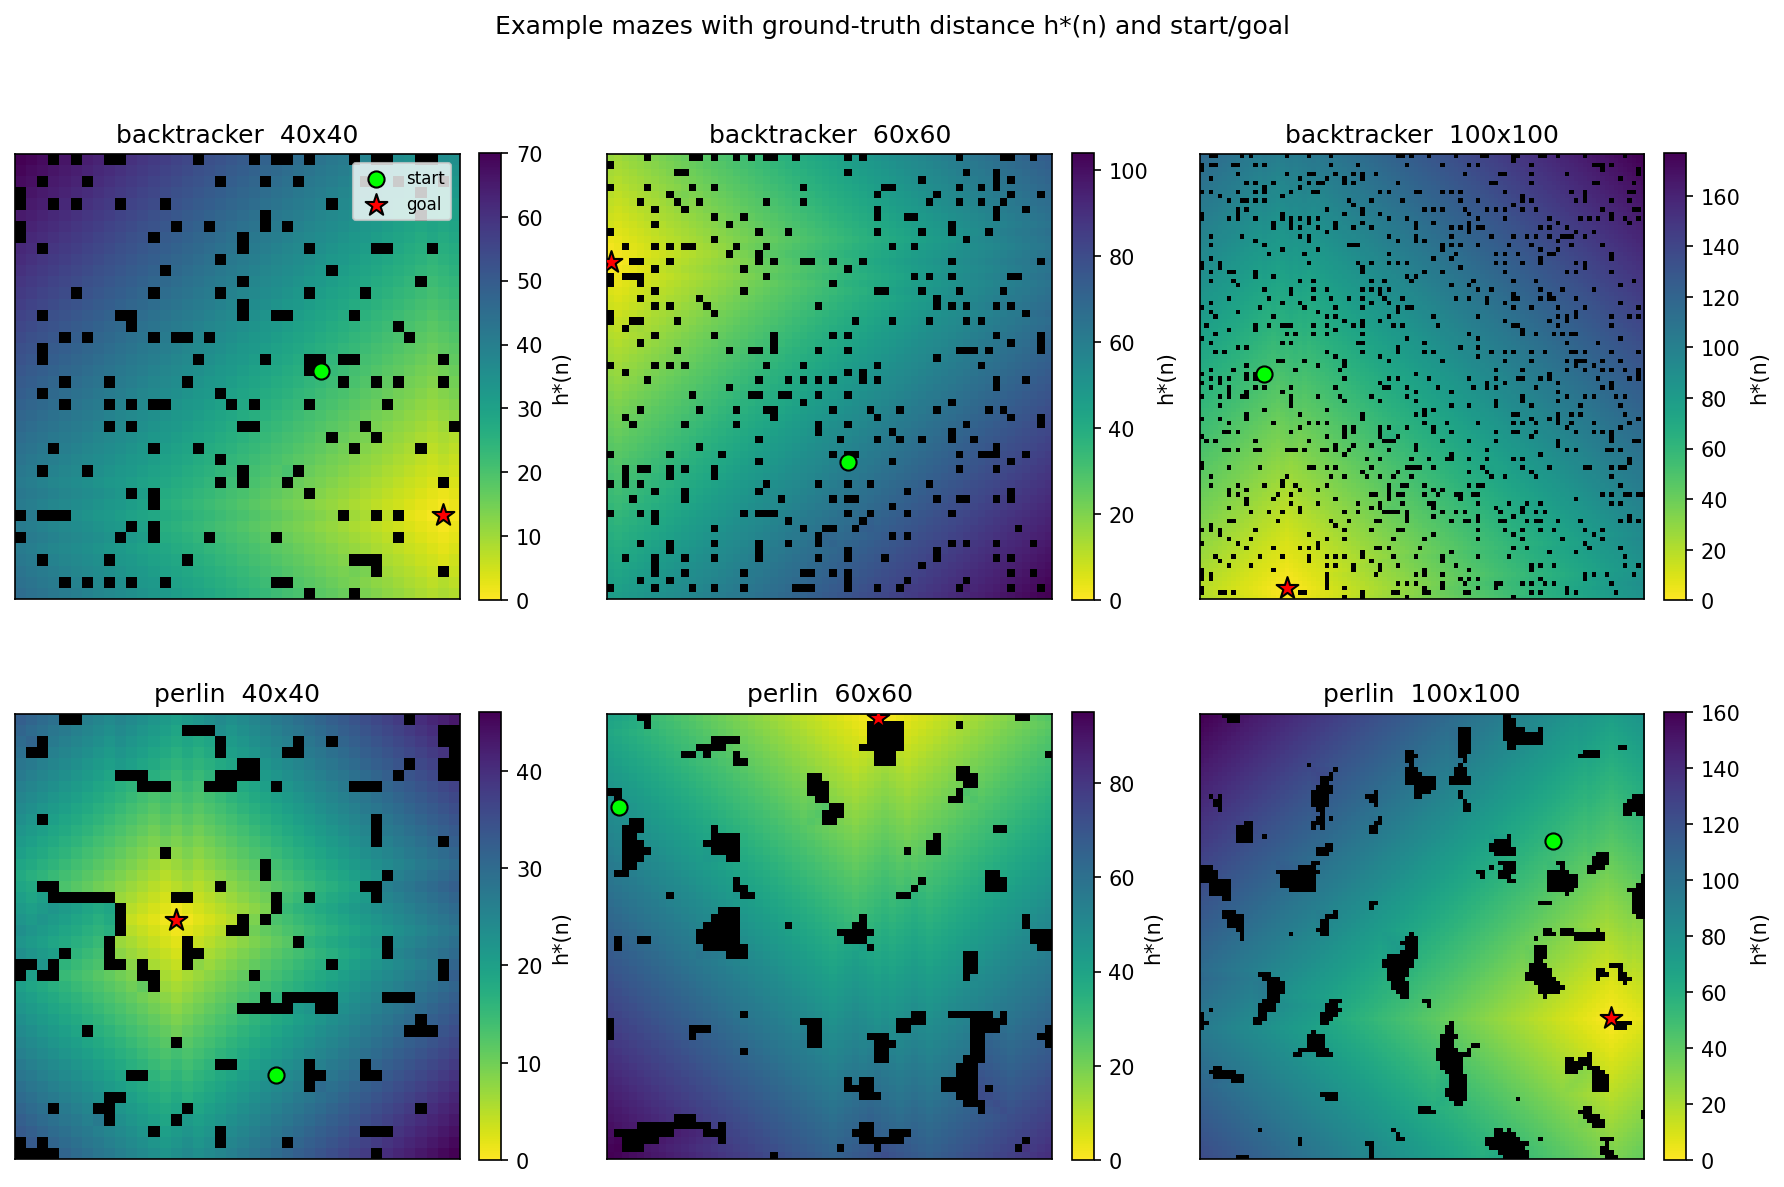
\includegraphics[width=\textwidth]{06_sample_mazes.png}
\caption{Example mazes (rows: generator; columns: size) with the ground-truth distance
field $h^\ast(n)$ and the start (circle) and goal (star).}
\label{fig:samples}
\end{figure}

\subsection{Cleaning Summary}
Figure~\ref{fig:cleaning} visualises the cleaning funnel of
Section~\ref{sec:cleaning}: from 2{,}000 generated mazes, 88 are removed for unreachable
goals, none are duplicates, and 36 are IQR outliers, leaving 1{,}876.

\begin{figure}[H]
\centering
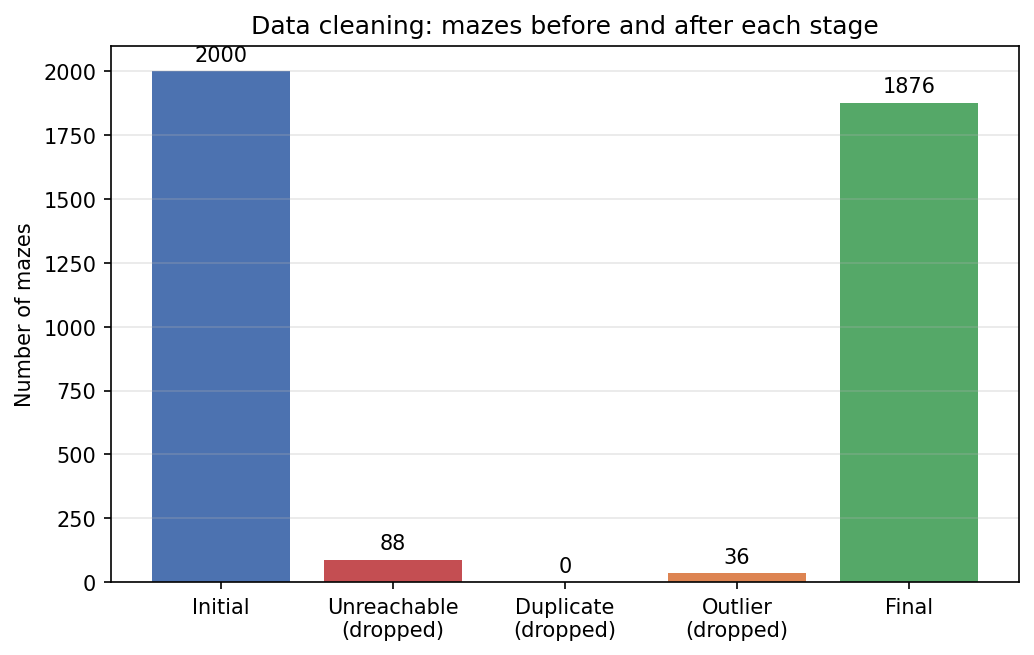
\includegraphics[width=0.68\textwidth]{07_cleaning_summary.png}
\caption{Maze counts before and after each cleaning stage.}
\label{fig:cleaning}
\end{figure}

\subsection{Feature Correlations}
Figure~\ref{fig:corr} shows the Pearson correlation matrix of the 29 input features. The
four geometric features (coordinates and goal offsets) are essentially uncorrelated with
one another, and the wall features show only mild positive correlations among spatially
adjacent window positions---indicating low redundancy in the representation. One feature,
the centre of the $5\times5$ window ($w_{2,2}$), is constant: it corresponds to the cell
itself, which is always free for emitted samples. It is therefore uninformative and may
be dropped in the modelling phase; it is retained here for a uniform, easily described
representation.

\begin{figure}[H]
\centering
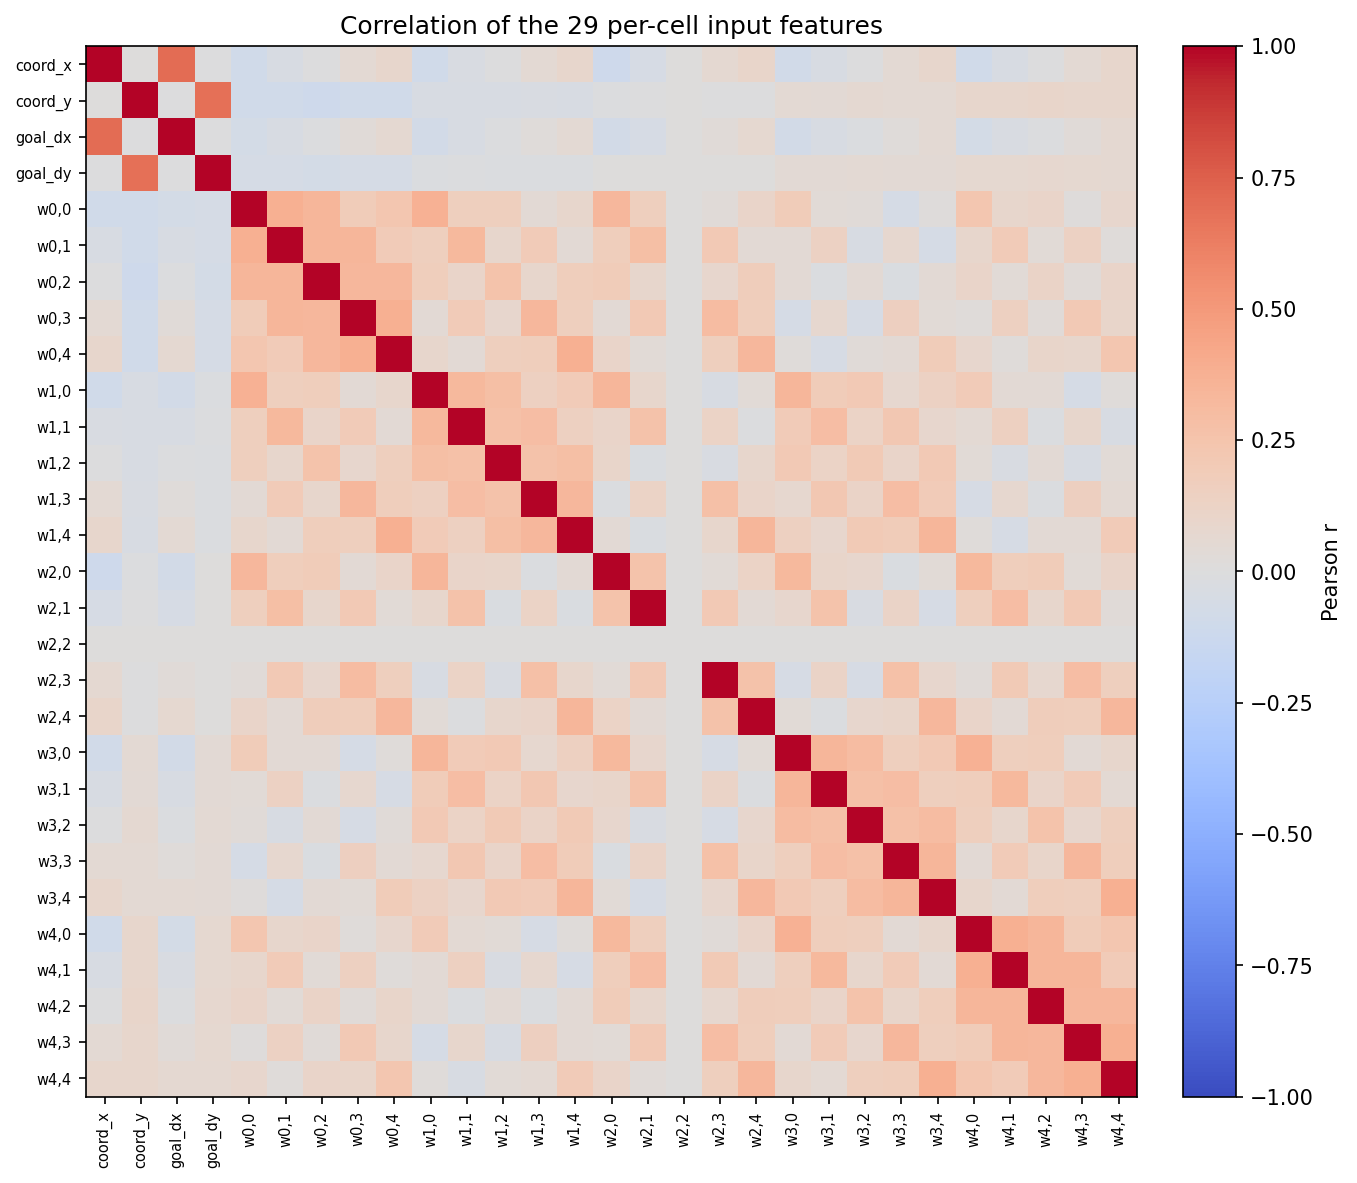
\includegraphics[width=0.82\textwidth]{08_feature_correlation.png}
\caption{Correlation matrix of the 29 per-cell input features.}
\label{fig:corr}
\end{figure}

% ===========================================================================
\section{Reproducibility}
% ===========================================================================
The full pipeline is deterministic given seed $42$ and runs in the following order:

\begin{verbatim}
python data_scripts/generate_mazes.py     # 2000 mazes  -> data/raw/
python data_scripts/compute_labels.py     # Dijkstra h* -> data/labeled/
python data_scripts/clean_data.py         # cleaning    -> data/cleaned/
python data_scripts/features.py           # features    -> data/processed/
python data_scripts/eda.py                # figures     -> figures/
\end{verbatim}

Generated data is written under \texttt{data/} and excluded from version control via
\texttt{.gitignore}; only scripts, logs, and figures are tracked.

% ===========================================================================
\section{Conclusion and Future Work}
% ===========================================================================
Deliverable~1 is complete on both fronts. Phase~1 articulates the problem, its
stakeholders, and a concrete argument for why learning the heuristic is the right
approach. Phase~2 delivers a fully reproducible, data-centric pipeline that produces
2{,}000 procedurally generated mazes, exact Dijkstra ground-truth labels, a cleaned
dataset of 1{,}876 mazes, a 29-dimensional per-cell feature representation with a
leakage-free split, and an exploratory analysis quantifying density fidelity,
connectivity, and feature structure.

The next deliverables implement the remaining research steps: (i) training the
feed-forward network to regress $h^\ast(n)/N$; (ii) integrating $h_\theta$ into A$^\ast$;
and (iii) evaluating nodes expanded, path-optimality ratio, and per-move latency against
Manhattan A$^\ast$ and the exact oracle heuristic---thereby testing the project's central
hypothesis.

% ===========================================================================
\begin{thebibliography}{9}
\bibitem{hart1968}
P.~E. Hart, N.~J. Nilsson, and B.~Raphael,
``A Formal Basis for the Heuristic Determination of Minimum Cost Paths,''
\emph{IEEE Transactions on Systems Science and Cybernetics}, vol.~4, no.~2, pp.~100--107, 1968.

\bibitem{dijkstra1959}
E.~W. Dijkstra,
``A Note on Two Problems in Connexion with Graphs,''
\emph{Numerische Mathematik}, vol.~1, pp.~269--271, 1959.

\bibitem{yonetani2021}
R.~Yonetani, T.~Taniai, M.~Barekatain, and J.~Fujimura,
``Path Planning using Neural A* Search,''
in \emph{Proc. International Conference on Machine Learning (ICML)}, 2021.
\end{thebibliography}

% ===========================================================================
\appendix
\section{Repository Structure}
% ===========================================================================
\begin{verbatim}
.
|-- README.md
|-- requirements.txt
|-- data_scripts/
|   |-- generate_mazes.py     # Phase 2: maze generation + generation_log.json
|   |-- compute_labels.py     # Phase 2: Dijkstra ground-truth labels
|   |-- clean_data.py         # Phase 2: cleaning (unreachable, dup, IQR)
|   |-- features.py           # Phase 2: 29-dim features + 70/15/15 split
|   `-- eda.py                # Phase 2: EDA figures
|-- figures/                  # EDA charts used in this report
|-- data/                     # generated data (git-ignored)
`-- report/
    |-- main.tex
    `-- Neural_Heuristic_Research.pdf
\end{verbatim}

\end{document}
